\chapter{Introduction}\label{ch:introduction}
\section{Problem statement}
In order for \ac{ML} systems to be used more widely,
they have to become more trustworthy \citep{hleg2019ethics}.
The susceptibility of deep \acp{NN} to adversarial attacks has been well documented, but there are other problems as well.
This includes their opaqueness and their general tendency to take shortcuts;
leading to situations where neural networks do not do `what we meant', but just what they were explicitly told to do.

This problem becomes especially severe when the training data is biased in some way,
which, by default, makes the \ac{ML} system internalise the bias, or, in some cases, even exacerbate it.
Consequently, when applied in the deployment setting, the system will not behave in the desired way.
The topic of this thesis is dealing with biased data,
where the bias is inextricably linked to a special attribute $s$.
% and what types of biases exist and how to correct them if possible.

\section{Motivation and aims}
Many datasets with person-related features display biases when examined by common fairness criteria.
This can range from relatively harmless biases,
like men being, on average, older than women in the CelebA dataset \citep{liu2015faceattributes},
to more serious ones,
like black men being several times less likely to receive bail than white men in the COMPAS dataset \citep{angwin2016machine}.
In the absence of truly `fair' datasets, our methods have to be able to avoid these biases.

% Now, one possible objection here is:
% if those datasets are of such poor quality,
% then maybe we just should not train any \ac{ML} model on these and should not use them to make automated decisions?
% While this question is mostly beyond the scope of this document, let me offer some thoughts on this:
% It is true that even after the application of de-biasing techniques,
% the resulting models still should not be fully trusted,
% but they can still ease the burden of checking everything manually;
% similar to an email spam filter which is not perfect, but still very useful.
% Or, put another way, it is always important to check what the realistic alternative is;
% we should not compare a model to a non-existing perfect ideal, but to the actual solution that would be used instead.
% One could imagine a hybrid approach where an automated system makes preliminary decisions,
% but random samples are reviewed by humans and decisions can always be challenged.
% Ideally, the model itself would tell us about decisions it is uncertain about.

% Moreover, two of the three methods presented in this thesis require access to (unlabelled) \emph{unbiased} data,
% which is used during the training process.
% The remaining method requires summary statistics of the unbiased target dataset.
% So, the criticism that we are only learning from biased data does not apply here.
% This should allow us to be more confident in the predictions produced by those methods,
% because the methods learn from additional, unbiased information.

Throughout this thesis, the aim is to learn a model from biased training data,
which gives fair predictions (where `fair' is given by specific definitions) on an unbiased test set.
It is thus not sufficient to simply optimise the cross-entropy on the training set;
we have to change the optimisation target to achieve our stated goal.
While it is possible to extend notions of fairness beyond classification tasks,
the vast majority of work in this area concerns classification only and that will be the case here as well.

This thesis will discuss two kinds of dataset bias: \emph{label bias} and \emph{sampling bias}.
In both cases,
we consider a classification problem in which the class labels $y$ need to be predicted from input features $\vx$.

In all cases, there is a special attribute $s$ associated with each input.
This attribute can have different meanings:
In the setting of \emph{label bias}, $s$ usually encodes membership in a demographic group, such as gender,
but more generally, it is a feature that should not be used to make predictions for legal or ethical reasons.
(See below for other possible meanings of $s$.)
In this setting, we call $s$ the \emph{sensitive attribute} (because it carries sensitive information).
We will often refer to the set of all samples which share a specific sensitive attribute as one \emph{demographic group}.
In most of the examples, $s$ and $y$ are binary variables, but this does not have to be the case.
Crucially, however, the label bias is related to $s$ in a very specific way:
depending on the value of $s$, labels are either flipped from $y=0$ to $y=1$ or vice versa,
\ie, there is an error in the labels which is correlated with the sensitive attribute.
This could, for example, be result of societal discrimination of demographic groups.

For \emph{sampling bias},
there is also a special attribute $s$, but it does not necessarily have to denote a \emph{sensitive} attribute;
it can more generally be a \emph{spurious} variable which is correlated with the class label $y$ in the training set,
but is not truly predictive of $y$ in the general case.
Alternatively, it might refer to a natural \emph{subgroup} of the $y$ classes.
Sampling bias then means that the training set is not uniformly sampled from the underlying distribution:
Instead, sampling depends on $s$ and $y\,$;
\eg, there might be almost no samples of $s=0$ and $y=1$ in the training set.
The effect is that \ac{ML} models are tempted to take shortcuts and use $s$ as a shorthand for $y$.

\Figref{fig:dataset-bias-overview} shows a visual representation of the two kinds of dataset bias discussed here.

\begin{figure}[tp]
  \centering
  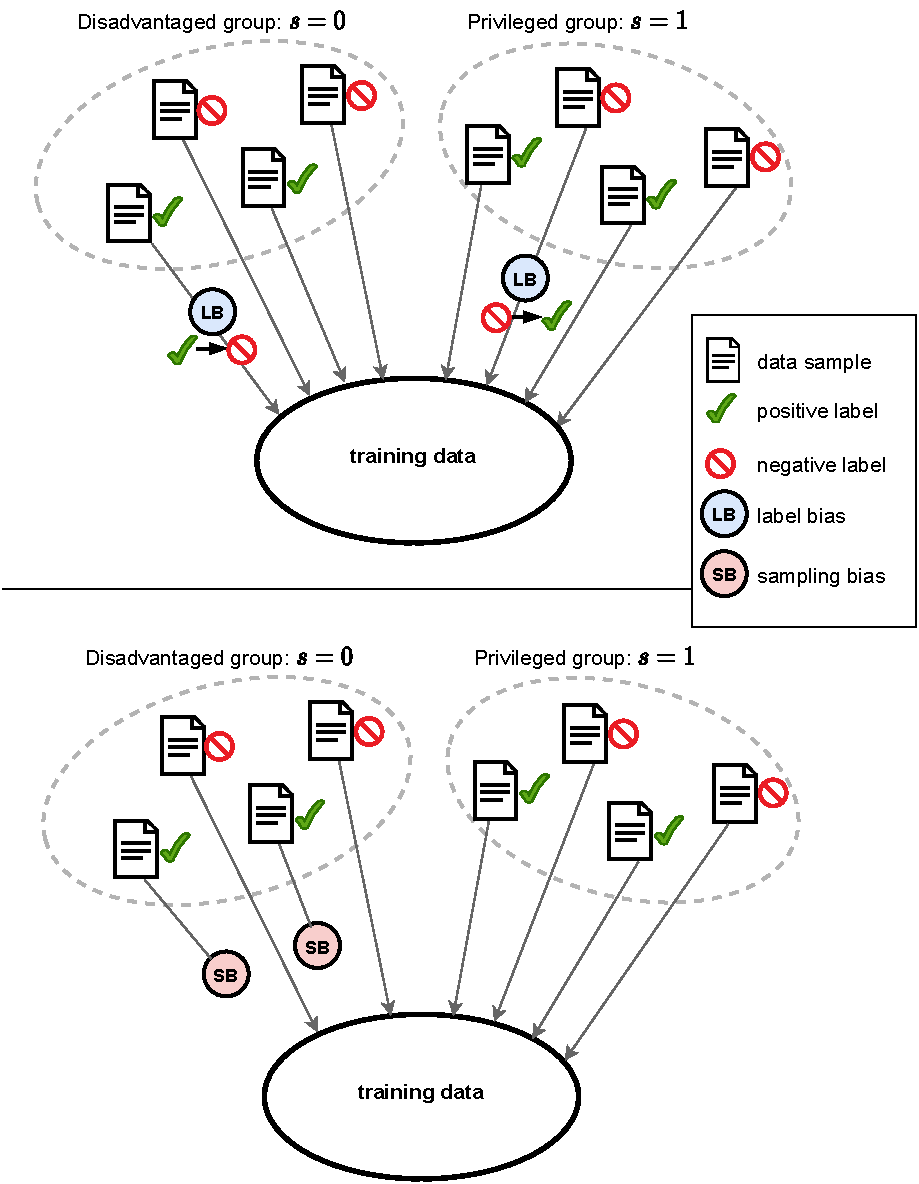
\includegraphics[width=\textwidth]{figures/dataset_bias_overview_vertical.pdf}
  \caption{%
    Schematic representation of label bias and sampling bias.
    \textsc{Top}: the label bias changes positive labels to negative labels for \(s=0\),
    and in the opposite direction for \(s=1\) (though this not always the case).
    \textsc{Bottom}: the sampling bias \emph{intercepts} samples with a positive label from \(s=0\).
  }%
  \label{fig:dataset-bias-overview}
\end{figure}

The overall goal in all cases is to make the classifier invariant to $s$.
We can measure the invariance to $s$ directly by computing \emph{fairness metrics}
for the predictions of the classifier.
In contrast to the accuracy metric,
these fairness metrics give a more complete picture of how invariant the classifier is.
This is especially true if evaluation is done on an imbalanced set
-- for example in the event that a truly unbiased test set is unavailable.
In such cases, accuracy can be highly misleading,
because good performance on the majority class can hide poor performance on a minority class.
Fairness metrics do not suffer from this problem
because they specifically look at the results in the different subgroups.
However, we typically try to evaluate our models on a test set that is as unbiased as possible,
in order for accuracy to be meaningful.

Fairness metrics require a fairness \emph{definition},
and the fairness definition with the clearest interpretation in the described setup of label bias and sampling bias is \acfi{DP},
also called \emph{statistical parity} or \emph{independence}.
It demands that the predictions $\hat{y}$\, be independent of the sensitive attribute \(s\).
So, for binary $s$ and $y$\,:
\begin{align}
  P(\hat{y}=1|s=0) &= P(\hat{y}=1|s=1)~.
  \label{eq:dp-def}
\end{align}
There are multiple \ac{DP} \emph{metrics} which track how close the predictions are to satisfying the equality,
among them, the difference and the ratio of the terms on the two sides of the equation.

When talking about \emph{un}biased datasets above,
we did not specify exactly what this meant,
and that is because the definition thereof can differ from task to task,
but one way to define it is as a \emph{balanced} dataset where all combinations of $s$ and $y$ occur at the same rate:
\begin{align}
  \label{eq:balanced-dataset}
  P(y=0,s=0)=P(y=0,s=1)=P(y=1,s=0)=\dots
\end{align}
In such a dataset, we have $y \perp s$, and thus,
perfect predictions ($\hat{y}=y$) on this dataset will satisfy $\hat{y} \perp s$ and hence \ac{DP}.
We can conclude that perfect accuracy on a balanced test set implies \acl{DP}
(the reverse does not hold).
However, if a model's predictions satisfy \ac{DP} on a \emph{biased} dataset,
then they cannot be perfectly accurate with respect to that dataset's biased labels anymore,
which makes sense because the goal is to be accurate to the \emph{unbiased} dataset.
This leads to a fairness-accuracy trade-off on biased test sets.

The other two fairness definitions which are commonly used are \acfi{EOpp} and \acfi{EOdds},
which do not require the prediction $\hat{y}$ to be independent of $s$,
but they do require that the model makes equally high-quality predictions for all values of $s$.
Concretely, for \ac{EOpp}, the \acfip{TPR} need to be the same for all demographic groups
(again for binary $s$ and $y$):
\begin{align}
  \label{eq:eopp-def}
  P(\hat{y}=1|y=1,s=0) = P(\hat{y}=1|y=1,s=1)~,
\end{align}
which is also required by \ac{EOdds}, but \ac{EOdds} additionally requires the same of the \acp{TNR}:
\begin{align}
  P(\hat{y}=y'|y=y',s=0) = P(\hat{y}=y'|y=y',s=1)\quad\forall y'~.
  \label{eq:eodds-def}
\end{align}
Just like \ac{DP},
the fairness definitions \ac{EOpp} and \ac{EOdds} can help us evaluate
how much a classifier is affected by the bias in the training set.

\section{Relations to other fields and clarification of terms}
% \subsection{aka: Isn't this thesis actually about XY instead of fairness?}
This thesis is principally written from the perspective of algorithmic fairness,
but it touches on other fields as well, like \emph{domain shift} and \emph{causality}.
Furthermore, the thesis makes use of concepts like \emph{transferable representations}
and \emph{interpretability}.
I summarise the areas here and discuss their relevance to the presented work.

A domain shift is, in general, a change in the data distribution between the training set and the deployment setting;
one often talks of a ``source domain'' and a ``target domain''.
Typically, this leads to poor performance of the \ac{ML} system in the deployment setting,
which necessitates the development of \emph{domain adaptation} methods.
There are thus strong parallels to the problem of dataset bias and fairness,
but domain shift is more general and has a different emphasis.
In domain shift, it is the whole data distribution that changes, including the meaning of individual features,
whereas in the biased-data setting (as defined in this thesis), the distribution of training data broadly matches that of the deployment setting, except for incorrect labels or censored sampling.
Furthermore, the field of algorithmic fairness is characterised by a focus on special attributes (sensitive attributes) that should not be used to make predictions;
a focus that the problem of domain shift lacks.
Nevertheless, methods developed for domain adaptation can often be adapted to the problem of biased data:
A not insignificant amount of the prior work discussed in \chapref{ch:related-work} was motivated by domain adaptation instead of fairness.
Similarly, it should be possible to adapt fairness methods to tackle domain shift,
however, this has rarely happened.

A related area is \emph{transfer learning},
which is usually summarised as:
learning on one task and transferring the knowledge to a different task.
The transfer can happen without any additional training (zero shot),
or, more commonly, with fine-tuning on a small (few shot) or large amount of additional data.
Transfer learning is not a direct goal of this thesis,
but learning \emph{transferable representations} is,
which is a much narrower goal.
In the context of this thesis,
transferable representations are understood to be representations of input features
that are (ideally) suitable for \emph{all} tasks that the original data is suitable for,
except for predicting the sensitive\slash spurious attribute \(s\).
This is in contrast to representations that are only useful for predicting one specific target.

The other closely related topic is \emph{causality}.
The argument that a solution to the dataset bias problem involves causality goes as follows:
As mentioned above, the goal is to ignore the bias in the data
and learn the true underlying structure that is hidden in the data.
Often, the most fundamental structure that we can learn is the \emph{causal} structure of the problem of interest.
For example, if an \acs{ML} model truly understood what makes someone a good employee,
it would not need to rely on surface characteristics like whether the applicant's name sounds foreign.
% Learning such causal models is not yet completely in the realm of what today's \ac{ML} systems can achieve \citep{pearl2019seven},
% and will likely require a very large amount of data.
% (The models that perhaps come close to this are methods like unsupervised methods like GPT \citep{radford2018improving,radford2019language,brown2020language} that have been trained on enormous amounts of data.)
However, the work in this thesis is not presented under the banner of causality, for several reasons.
% First, a majority of the experiments are on images, such that the input features are pixel values,
% and thus do not lend themselves well to be analysed with methods like Bayesian
First, in as far as the presented methods solve a causal structure problem, they solve a very limited one;
inputs are mapped to outputs, and no detailed exploration of a potential implicit causal model is performed.
Second, the discovered robust structures are not necessarily \emph{causal} in nature, in a narrow sense of the word.
This is especially true in image data:
For example, while discovering that the presence of a smile and the gender of the person in a photograph are two distinct characteristics
requires a deep understanding of human faces,
it does not require knowing how smiles and gender are related via cause-and-effect in the real world.

In the chapter on related work (\chapref{ch:related-work}),
I discuss several methods that apply proper causal methods to fairness,
but those methods assume that the true causal structure of the problem is already known,
and are not helpful for discovering such structures.
To work properly, they need access to either Bayesian networks or structural equation models.
Neither of which the methods presented in this thesis can provide.

Finally, a note on the terms ``interpretability'' and ``explainability'' in the context of \ac{ML} and artificial intelligence:
many different definitions have been proposed \citep{barredoarrieta2020xai},
but no consensus has emerged yet on what these terms should mean.
In the context of this thesis, the term ``interpretable'' is applied to information,
and is taken to mean that these pieces of information are provided in a form that is readily understandable and inspectable by humans.
In this sense, a visualisation of an embedding or representation as an image in the original data domain
is interpretable,
but a 100-dimensional vector of floating point number is not.

\section{Structure of document}%
\label{sec:thesis-structure}
In \chapref{ch:related-work}, I present related work,
concentrating on the area of algorithmic fairness and dataset bias.
\Chapref{ch:content} summarises the main contributions of this thesis
and describes their relationship to one another.
The chapter concludes with a list of the publications that constitute the main contribution of the thesis,
accompanied by a description of the contributions to the publications, separated by author.
\Rangechapref{ch:paper1}{ch:paper3} reproduce these publications with minimal changes.
% constitute the main contribution of this thesis.
% Each of these chapters starts with a brief section which positions the chapter in the context of the this document.
% This is followed by the contents of publications.
In the final chapter, \chapref{ch:conclusion}, I present conclusions from the main work and directions for future work.
